\documentclass[12pt]{article}
\usepackage{graphicx}
\usepackage{wrapfig}
\usepackage{subfigure}
\usepackage{multirow}
\usepackage{hyperref}
\usepackage{amsmath}
\usepackage{amssymb}
\usepackage{ngerman}
\usepackage[ansinew]{inputenc}
\usepackage[left=2cm,top=1cm]{geometry}

% vector graphics test
\usepackage{color}
\usepackage{transparent}
\graphicspath{{graphs/}}

\setlength{\parindent}{0pt}

%\usepackage[outdir=./]{epstopdf}
%\epstopdfsetup{outdir=./}


\begin{document}
	\pagestyle{empty}
	

\begin{titlepage}
	\centering
	\bigskip
	\huge{Astronomisches Praktikum: Teleskope und Astrometrie}\\
	\bigskip
	\large{Versuch 6}\\
	\bigskip
	\large{Jan R\"{o}der \& Julia Lienert}
	\bigskip
	\tableofcontents
\end{titlepage}

\pagebreak


\section{Einleitung}



\section{Teleskope}

\subsection{Aufgabe 1}














\section{Abbildungsma"sstab}
\section{Abbildungsg\"{u}te}
\section{Astrometrie: Der Schnelll\"{a}ufer BD +18$\mathring{}$ 2776}




\pagebreak

\section{Diskussion}




\begin{figure} [h]
	\centering
	%	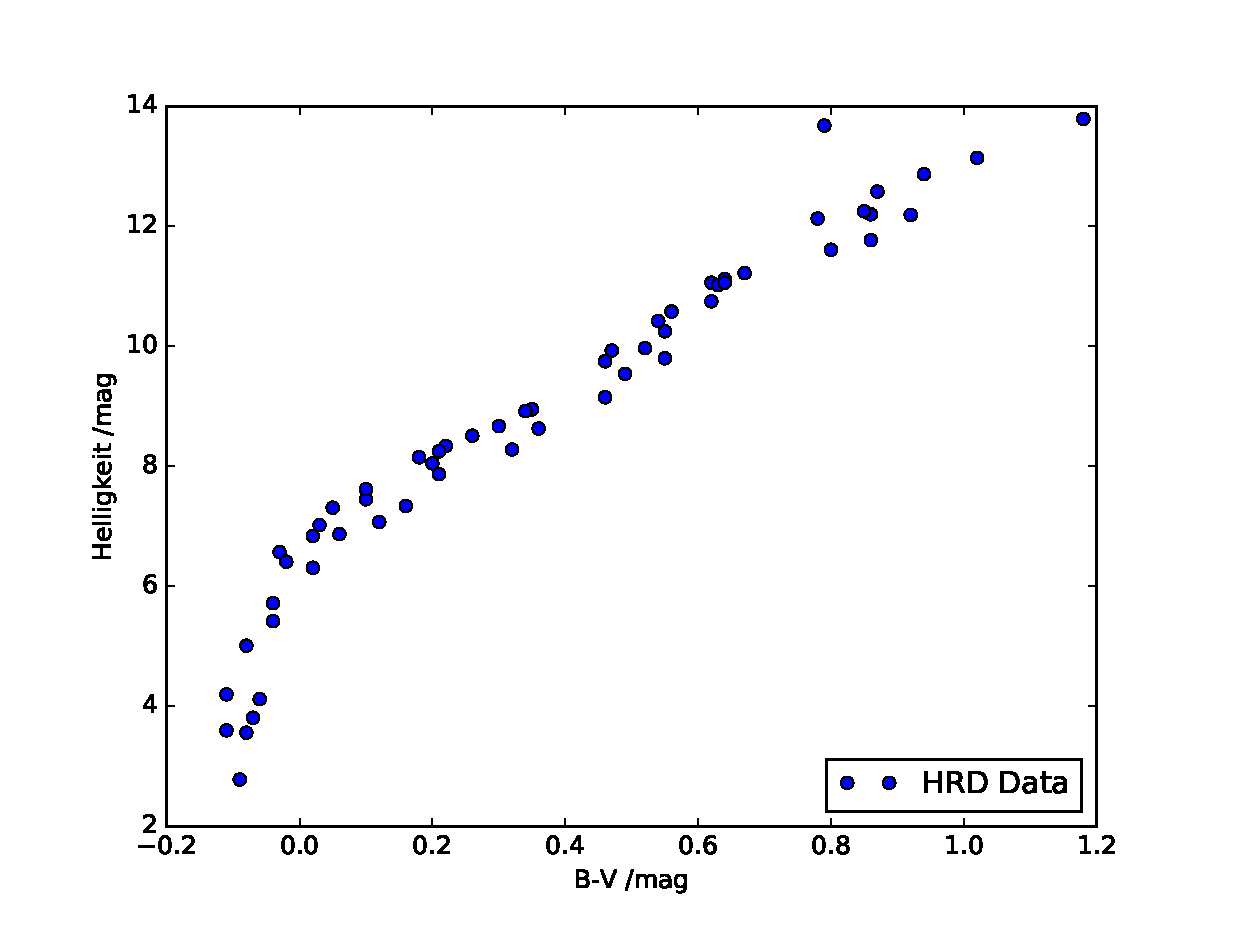
\includegraphics[width=1\textwidth]{hrd_notitle.eps}
	\caption{Scheinbare Helligkeit und Farbindex gegeneinander aufgetragen. Der rote Punkt w\"{a}re die Sonne, w\"{a}re sie Teil des Haufens.}
	\label{fig:hrd_unknown}
\end{figure}

















\end{document}